\documentclass{standalone}

\usepackage{tikz}
\usetikzlibrary{calc}

\begin{document}

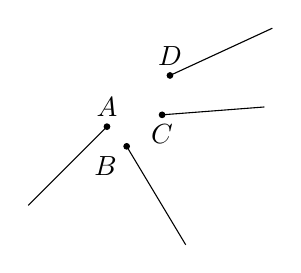
\begin{tikzpicture}[scale=1]

\coordinate (A1)  at (0,0);
\coordinate (A) at ($(A1)+(1,1)$);
\coordinate (B1)  at (2,-0.5);
\coordinate (B) at ($(B1)+(-0.75,1.25)$);
\coordinate (C1)  at (3,1.25);
\coordinate (C) at ($(C1)+(-1.3,-0.1)$);
\coordinate (D1)  at (3.1,2.25);
\coordinate (D) at ($(D1)+(-1.3,-0.6)$);

\foreach \pt/\pos in {A/above,B/below left,C/below,D/above}{
	\draw (\pt)--(\pt1);
	\draw[fill=black] (\pt) circle (1pt) node[\pos] {$\pt$};
}

\end{tikzpicture}

\end{document}